\documentclass[conference]{IEEEtran}

\usepackage{cite}
\usepackage{amsmath,amssymb,amsfonts}
\usepackage{algorithmic}
\usepackage{graphicx}
\usepackage{textcomp}
\usepackage{booktabs}
\usepackage{multirow}
\usepackage{xcolor}
\usepackage{hyperref}
\usepackage{balance}

\def\BibTeX{{\rm B\kern-.05em{\sc i\kern-.025em b}\kern-.08em
    T\kern-.1667em\lower.7ex\hbox{E}\kern-.125emX}}

\begin{document}

\title{Budget-Aware Sampling Strategies for Multi-Objective Optimization in Software Engineering}

\author{
\IEEEauthorblockN{[Author Name]}
\IEEEauthorblockA{[University Name]\\
[City, State]\\
[email]}
}

\maketitle

\begin{abstract}
In software engineering, many decisions involve optimizing multiple conflicting objectives simultaneously. Evaluating every possible configuration is expensive. If practitioners can only afford to evaluate a small sample (5--30\%) of all configurations, which sampling strategy should they use to build a surrogate model that best approximates the true Pareto front? We present the first systematic study comparing 7~sampling strategies and 3~baselines across 6~MOOT benchmark datasets at 4~budget levels with 20~repetitions (4,800 experiments total). Our key findings: (1)~objective-aware selection (NSGA-II, SWAY) outperforms surrogate-based methods in raw recall, but uses 3--100$\times$ more objective evaluations; (2)~among equal-budget methods, Diversity (MaxMin) is best overall (1.17--1.44$\times$ over random); (3)~the optimal surrogate strategy is budget-dependent---Stratified wins at 5\%, Diversity dominates at 10\%+; (4)~classical DoE methods (LHS, Sobol) \emph{fail} on discrete SE data, performing worse than random.
\end{abstract}

\begin{IEEEkeywords}
multi-objective optimization, sampling strategies, surrogate modeling, software engineering, Pareto front, design of experiments
\end{IEEEkeywords}

%===================================================================
\section{Introduction}
\label{sec:intro}

In software engineering, critical decisions often require balancing multiple conflicting objectives simultaneously---for example, minimizing cost while maximizing quality and minimizing delivery time. These are inherently multi-objective optimization (MOO) problems where the goal is to find the \emph{Pareto front}: the set of solutions where no objective can be improved without degrading another.

Evaluating every possible configuration is often prohibitively expensive. \emph{Surrogate-assisted optimization} addresses this by training a machine learning model on a small subset of evaluated configurations and predicting objectives for unevaluated ones. This raises a critical question:

\emph{If you can only afford to evaluate a small sample (5--30\%) of all configurations, which sampling strategy should you use to build a surrogate model that best approximates the true Pareto front?}

This question sits at the intersection of three research areas---surrogate modeling, sampling/Design of Experiments (DoE), and multi-objective software engineering---yet has received almost no systematic study (Section~\ref{sec:gap}). Classical DoE methods (Latin Hypercube Sampling, Sobol sequences) were designed for continuous engineering spaces, not the discrete, mixed-type data common in SE.

\textbf{Contributions.} We present a systematic empirical study comparing 7~sampling strategies plus 3~baselines across 6~MOOT benchmark datasets at 4~budget levels (5\%, 10\%, 20\%, 30\%), with 20~repetitions per configuration (4,800 total experiments):

\begin{enumerate}
    \item Objective-aware baselines (NSGA-II at 0.500 mean recall, SWAY at 0.421) outperform all surrogate methods---but use 3--100$\times$ more evaluations.
    \item Among equal-budget surrogate methods, Diversity (MaxMin) is best overall (0.279 mean recall, 1.17--1.44$\times$ over random).
    \item The optimal surrogate strategy is \emph{budget-dependent}: Stratified wins at 5\%, Diversity dominates at 10\%+.
    \item Classical DoE methods (LHS, Sobol) \emph{fail} on discrete SE data.
\end{enumerate}

%===================================================================
\section{Literature Review}
\label{sec:lit}

\subsection{Surrogate-Assisted Optimization}
Jin~\cite{jin2003} established surrogate modeling for evolutionary optimization. In SE, Ha \& Zhang~\cite{ha2019deepperf} used deep neural networks for performance prediction, while Nair et al.~\cite{nair2018flash} applied spectral learning for configuration performance models. Guo et al.~\cite{guo2018} studied data-efficient performance learning. These demonstrate surrogates' effectiveness but don't compare sampling strategies.

\subsection{Sampling / Design of Experiments}
Bergstra \& Bengio~\cite{bergstra2012} showed random search outperforms grid search for hyperparameter optimization. Chen et al.~\cite{chen2019sampling} introduced SWAY, showing sampling can match evolutionary algorithms. Nair et al.~\cite{nair2017bad} and Jamshidi et al.~\cite{jamshidi2018} explored sampling for configuration learning.

\subsection{Multi-Objective SE}
Sayyad et al.~\cite{sayyad2013} pioneered MOO for software product lines. Henard et al.~\cite{henard2015} combined search with constraint solving for SPL configuration. Wang et al.~\cite{wang2016} provided guidance on quality indicators for SBSE.

\subsection{Active Learning for Optimization}
Zuluaga et al.~\cite{zuluaga2013} proposed PAL for MOO via active learning. Krall et al.~\cite{krall2015gale} introduced GALE for geometric active learning in SBSE. Lustosa \& Menzies~\cite{lustosa2024,lustosa2025} explore noise reduction and partial ordering for model-based SE reasoning.

%===================================================================
\section{Research Gap}
\label{sec:gap}

We analyzed 60+ papers from MOOT citations and domain literature, applying knee-point analysis to identify the most influential works. We identified five thematic groups: (A)~Surrogate/Model-based, (B)~Sampling/DoE, (C)~Software Config/SE, (D)~Active Learning, (E)~MOO Algorithms. The full intersection $A \cap B \cap C = \emptyset$---no prior work systematically compares sampling strategies for training surrogates on discrete SE data.

\begin{figure}[htbp]
    \centering
    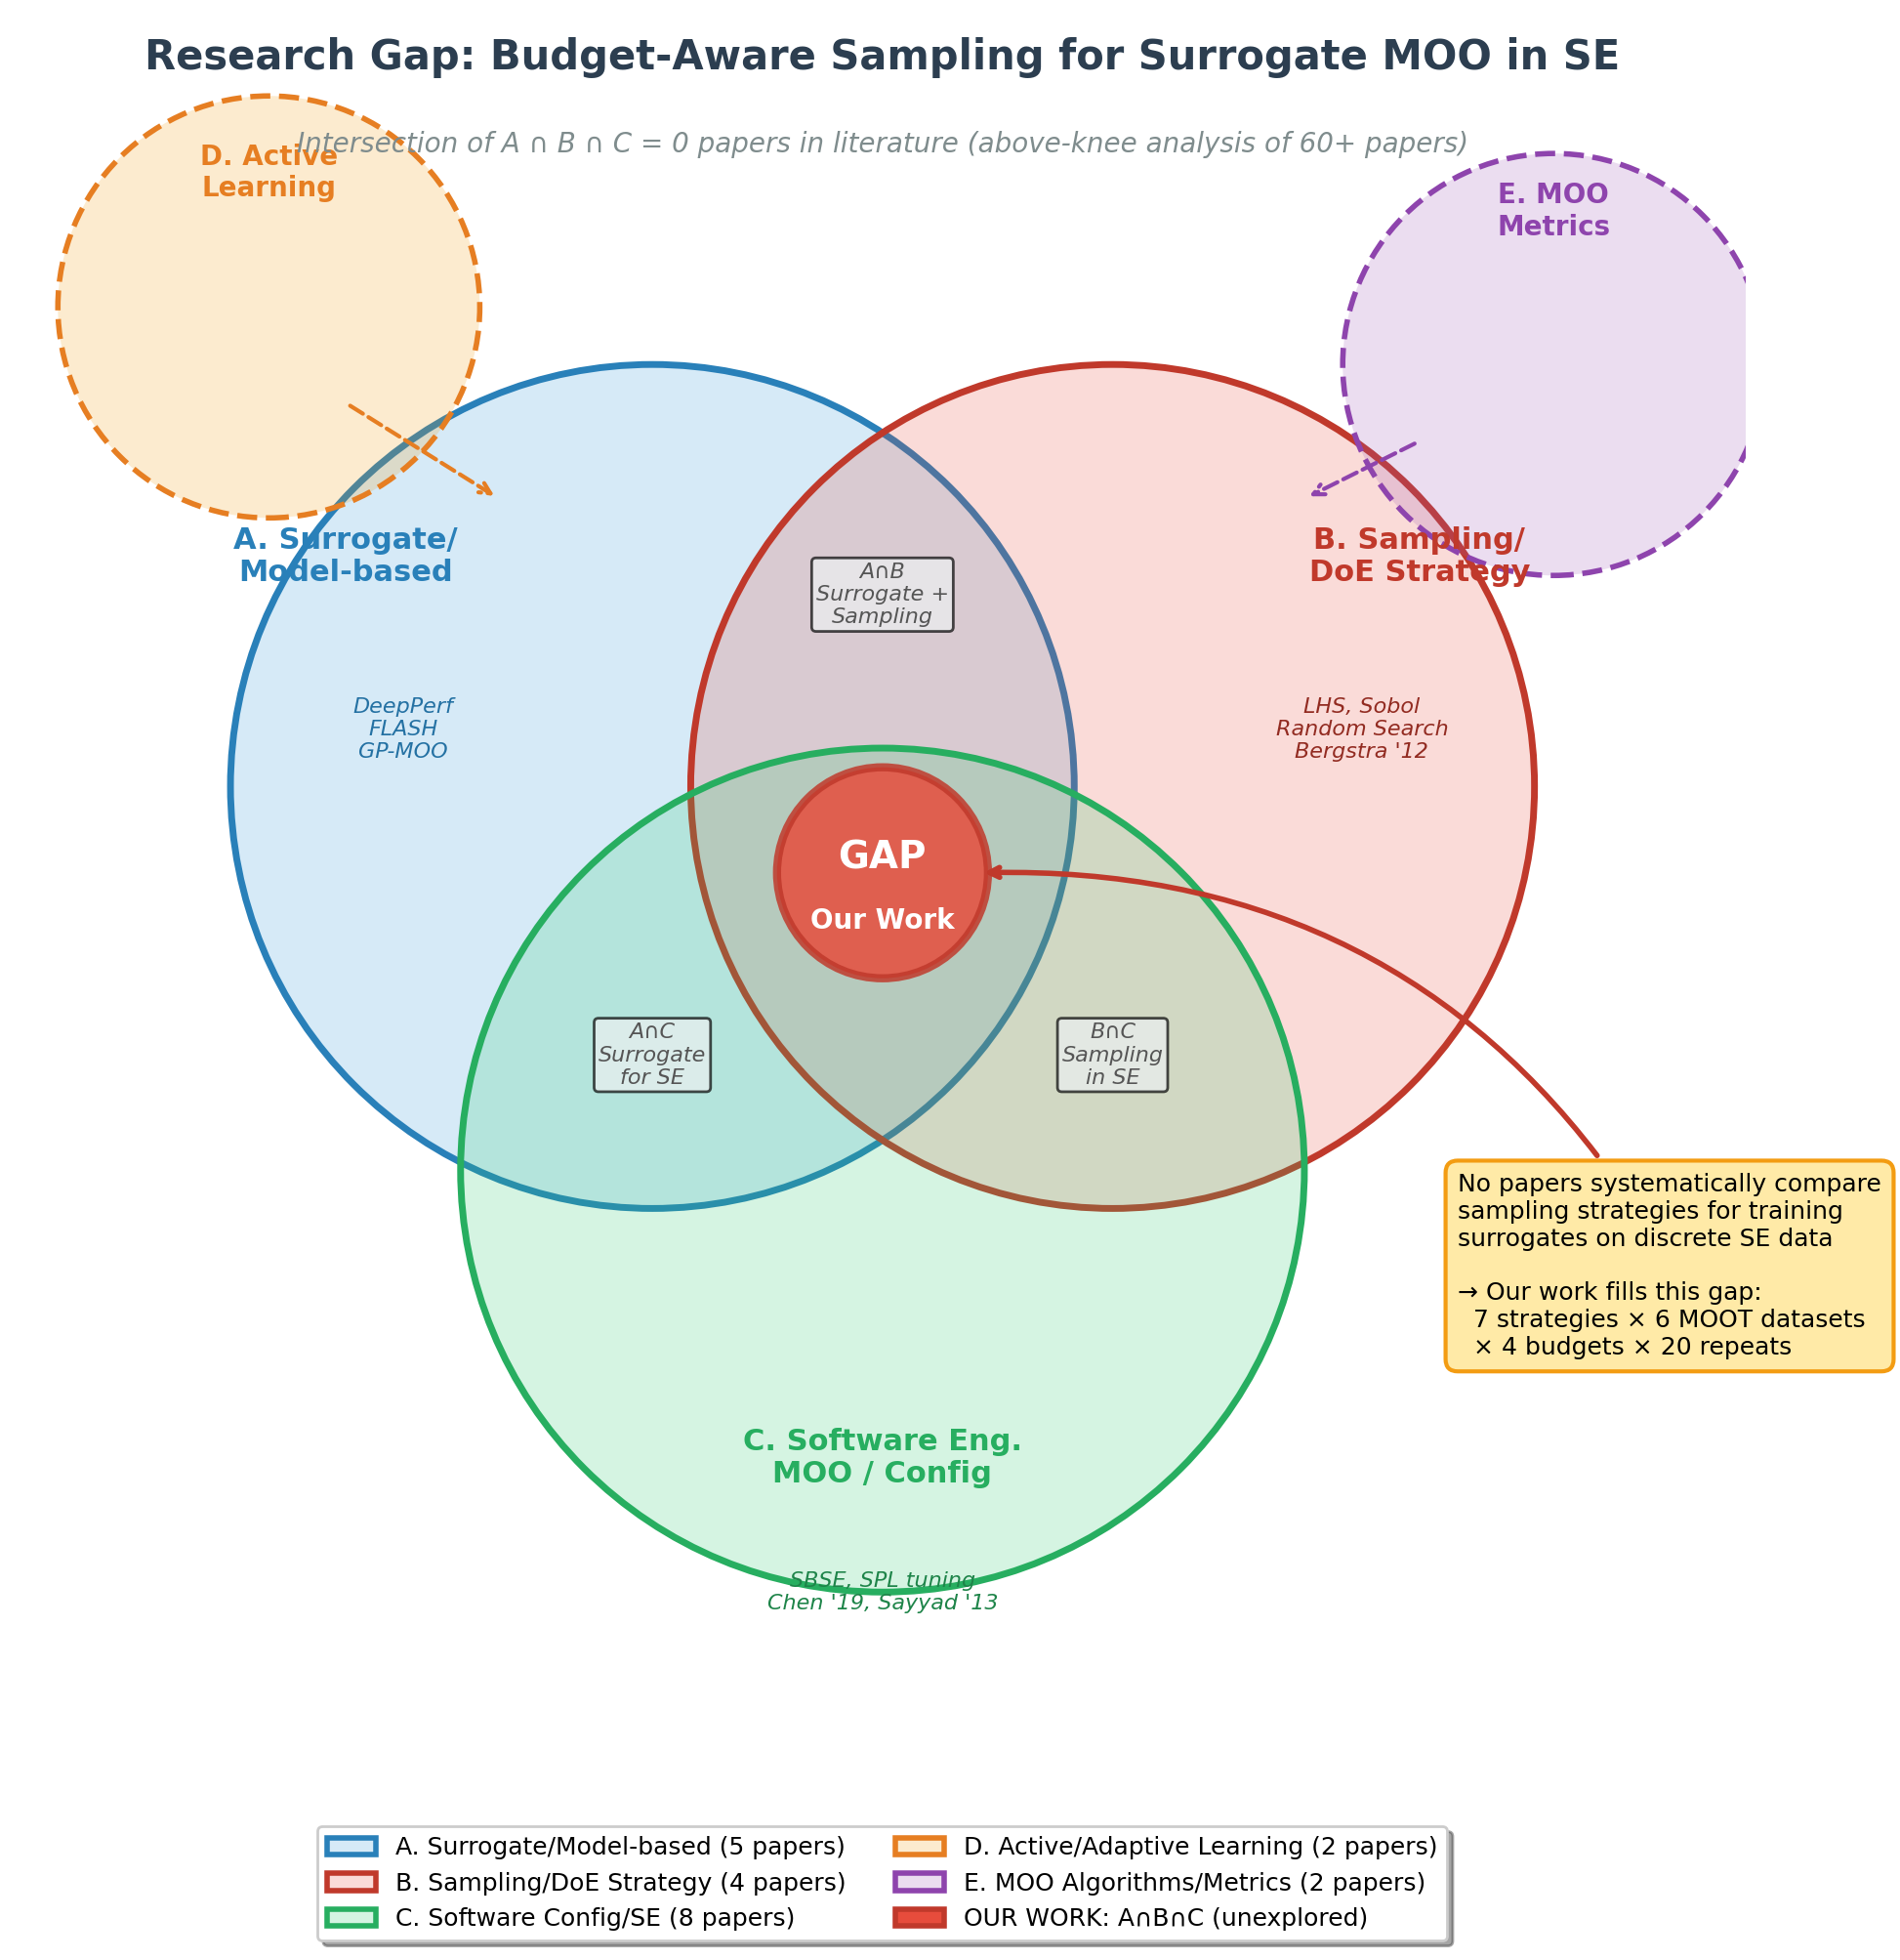
\includegraphics[width=\columnwidth]{venn_research_gap.png}
    \caption{Research gap Venn diagram. Five thematic groups from above-knee analysis. The center ($A \cap B \cap C$) is unexplored.}
    \label{fig:venn}
\end{figure}

%===================================================================
\section{Methodology}
\label{sec:method}

\subsection{Datasets}

We select 6 datasets from the MOOT benchmark repository~\cite{moot}:

\begin{table}[htbp]
\caption{Dataset Characteristics}
\label{tab:datasets}
\centering
\begin{tabular}{lrrrl}
\toprule
Dataset & Rows & Obj. & PF Size & Domain \\
\midrule
auto93 & 398 & 3 & 13 (3.3\%) & Automotive \\
pom3d & 500 & 3 & 7 (1.4\%) & Project mgmt \\
SS-A & 1,343 & 2 & 3 (0.2\%) & Configuration \\
SS-B & 206 & 2 & 2 (1.0\%) & Configuration \\
Wine\_quality & 1,599 & 2 & 4 (0.3\%) & Miscellaneous \\
coc1000 & 1,000 & 5 & 144 (14.4\%) & Cost estimation \\
\bottomrule
\end{tabular}
\end{table}

\subsection{Pipeline}

For each (dataset, method, budget, repeat): (1)~parse MOOT CSV, (2)~encode categorical features, (3)~sample $X\%$ of rows, (4)~train RandomForestRegressor (100 trees, multi-output), (5)~predict objectives for unseen rows, (6)~compute predicted Pareto front from combined values, (7)~evaluate against true PF.

\subsection{Sampling Strategies}

\begin{enumerate}
    \item \textbf{Random}: uniform random without replacement
    \item \textbf{Stratified}: bin first objective into $\sqrt{n}$ strata, sample proportionally
    \item \textbf{Clustering}: KMeans into $k$ clusters, pick nearest-to-centroid
    \item \textbf{Diversity (MaxMin)}: iteratively pick farthest point from selected set
    \item \textbf{LHS}: Latin Hypercube design mapped to nearest data points
    \item \textbf{Sobol}: quasi-random sequence mapped to nearest data points
    \item \textbf{Active Learning}: 20\% seed + iterative uncertainty sampling (RF variance)
\end{enumerate}

\subsection{Baselines}

\begin{enumerate}
    \item \textbf{NoModel}: compute PF of random sample only (no surrogate)
    \item \textbf{SWAY}~\cite{chen2019sampling}: recursive random projections, keep better half
    \item \textbf{NSGA-II}: non-dominated sorting + crowding distance on 3$\times$ budget pool
\end{enumerate}

\subsection{Metrics}

\begin{itemize}
    \item \textbf{Pareto Recall}: fraction of true PF found in predicted PF
    \item \textbf{Pareto Precision}: fraction of predicted PF that is truly optimal
    \item \textbf{IGD}: average minimum distance from true PF to predicted PF
    \item \textbf{HV Difference}: relative hypervolume difference
\end{itemize}

\subsection{Scale}

$7~\text{methods} \times 4~\text{budgets} \times 6~\text{datasets} \times 20~\text{repeats} = 3{,}360$ experiments, plus $3 \times 4 \times 6 \times 20 = 1{,}440$ baseline experiments.

%===================================================================
\section{Results}
\label{sec:results}

\begin{table}[htbp]
\caption{Best Method at Each Budget (Mean Recall)}
\label{tab:best}
\centering
\begin{tabular}{rllrl}
\toprule
Budget & Best Overall & Recall & vs Rand & Best Surrogate \\
\midrule
5\% & SWAY & 0.251 & 1.98$\times$ & Stratified (0.148) \\
10\% & SWAY & 0.322 & 1.94$\times$ & Diversity (0.224) \\
20\% & NSGA-II & 0.611 & 2.60$\times$ & Diversity (0.339) \\
30\% & NSGA-II & 0.909 & 2.76$\times$ & Diversity (0.406) \\
\bottomrule
\end{tabular}
\end{table}

\begin{table}[htbp]
\caption{Overall Method Ranking (Mean Recall Across All Budgets)}
\label{tab:ranking}
\centering
\begin{tabular}{rlrl}
\toprule
Rank & Method & Mean Recall & Type \\
\midrule
1 & NSGA-II & 0.500 & Baseline (3$\times$ eval) \\
2 & SWAY & 0.421 & Baseline (100\% eval) \\
\midrule
3 & Diversity & 0.279 & Surrogate \\
4 & Clustering & 0.228 & Surrogate \\
5 & Stratified & 0.223 & Surrogate \\
6 & Active Learning & 0.217 & Surrogate \\
7 & Random & 0.214 & Surrogate \\
\midrule
8 & NoModel & 0.158 & Baseline (X\% eval) \\
9 & LHS & 0.138 & Surrogate \\
10 & Sobol & 0.127 & Surrogate \\
\bottomrule
\end{tabular}
\end{table}

\textbf{Key findings:}

\emph{Objective-aware baselines dominate.} NSGA-II achieves 0.909 recall at 30\% budget, and SWAY leads at 5\% (0.251) and 10\% (0.322). However, NSGA-II evaluates 3$\times$ more rows' objectives, and SWAY uses all rows' objectives for binary splitting.

\emph{Among equal-budget methods, Diversity wins.} Restricting to methods that evaluate exactly $X\%$ of rows, Diversity (MaxMin) is best at 10\%+ and Stratified at 5\%.

\emph{DoE failure on discrete data.} LHS and Sobol perform worse than random (Table~\ref{tab:ranking}). These methods generate continuous points that map poorly to discrete data---multiple design points collapse to the same data row.

\emph{Surrogate vs.\ more evaluations.} All surrogate methods outperform NoModel (same budget, no model), confirming surrogate value. But NSGA-II and SWAY show that directly seeing more objective values can outperform model-based generalization---a cost--accuracy trade-off for practitioners.

\begin{figure}[htbp]
    \centering
    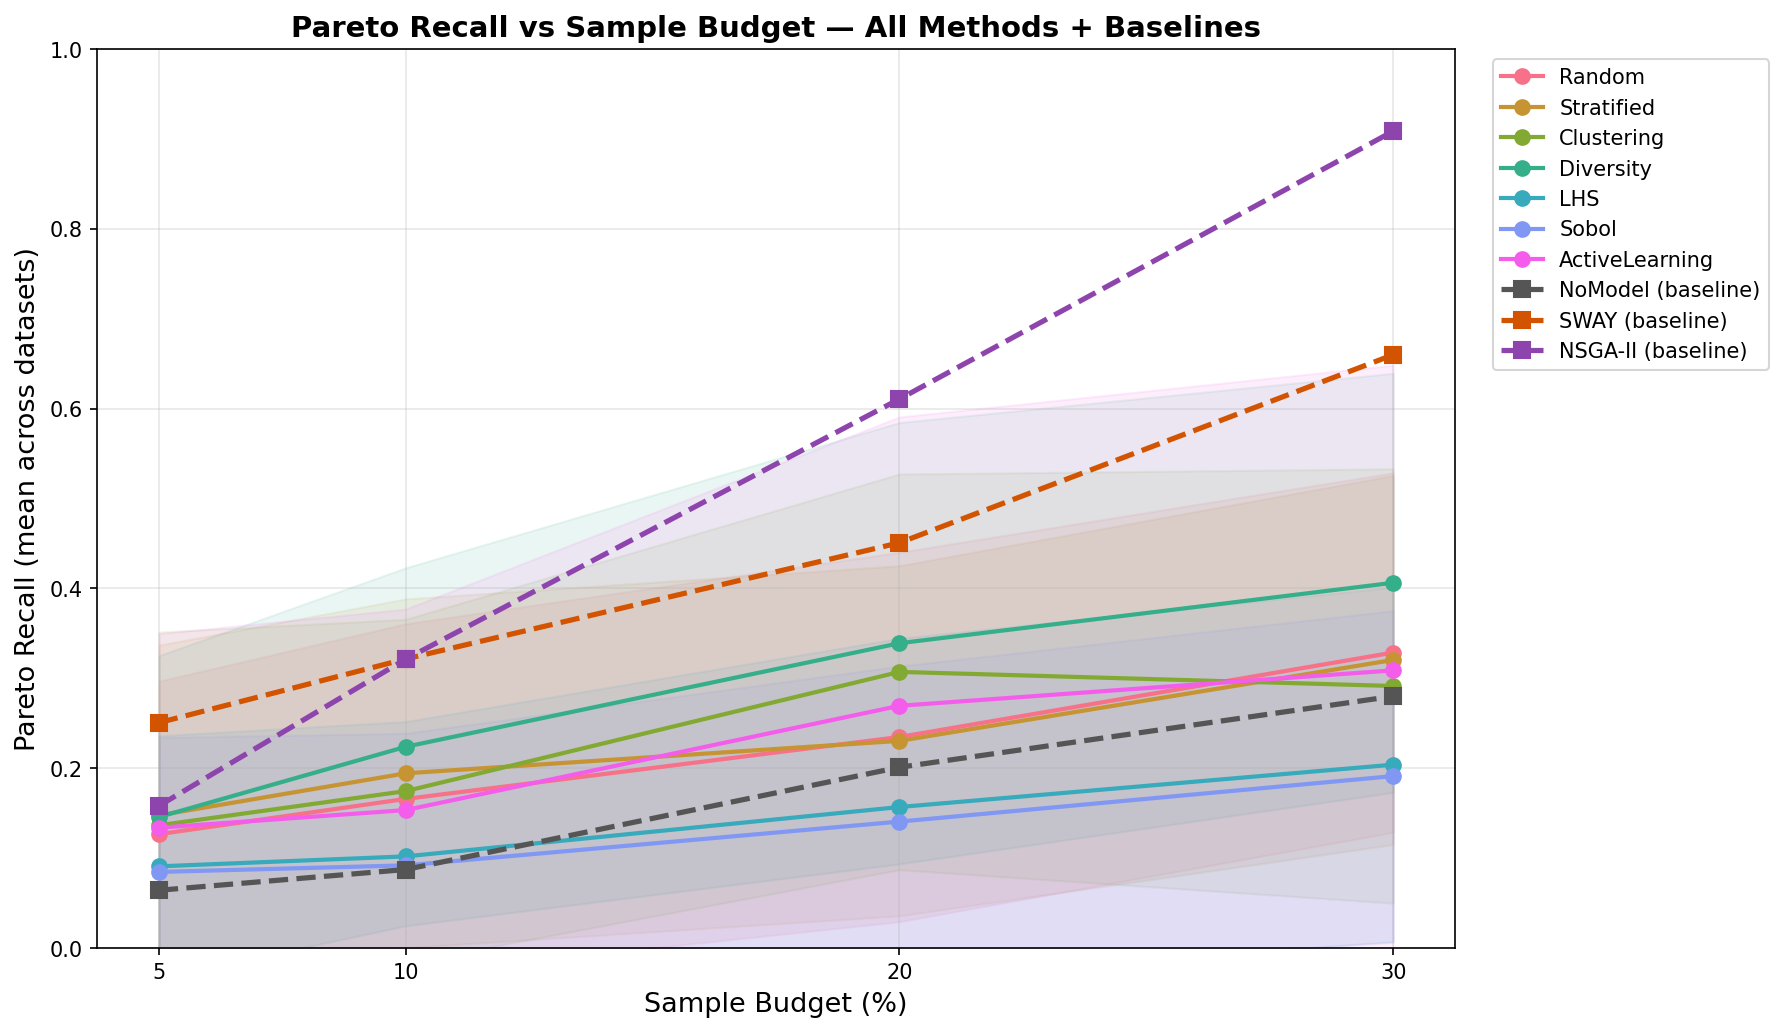
\includegraphics[width=\columnwidth]{results_recall_all_methods.png}
    \caption{Pareto Recall vs Sample Budget---all methods including baselines.}
    \label{fig:recall}
\end{figure}

%===================================================================
\section{Discussion}
\label{sec:discussion}

The results reveal a fundamental trade-off between \emph{evaluation budget} and \emph{model-based generalization}. NSGA-II and SWAY achieve superior recall by using more objective evaluations (3$\times$ and 100\%, respectively), but if objective evaluations are expensive, the surrogate approach evaluates only $X\%$ of rows and predicts the rest.

At 30\% budget, NSGA-II evaluates up to 90\% of rows (pool = $3 \times 30\%$) and achieves 0.909 recall. The best surrogate method (Diversity) evaluates only 30\% yet achieves 0.406 recall---lower, but using 3$\times$ fewer evaluations. When evaluation cost dominates, Diversity+surrogate is more efficient per evaluation.

SWAY's strong performance at low budgets (0.251 at 5\%) comes from using \emph{all} rows' objectives for recursive binary splitting~\cite{chen2019sampling}, effectively a 100\% evaluation budget. This is appropriate when objectives are cheap but optimization is the bottleneck.

The failure of LHS/Sobol on discrete data is an important practical finding. Practitioners defaulting to these standard DoE techniques for configurable software optimization would underperform random sampling.

%===================================================================
\section{Threats to Validity}
\label{sec:threats}

\emph{Internal:} We use Random Forest as the sole surrogate model. Other models (GP, neural networks) could yield different rankings. Seeds are deterministic with 20 repeats.

\emph{External:} 6 datasets from MOOT may not represent all SE optimization. Most have 2--3 objectives; results may differ for many-objective ($>$5) problems.

\emph{Construct:} Hypervolume uses Monte Carlo approximation for $>$2D. Baselines use different evaluation budgets: NSGA-II sees 3$\times$ budget rows, SWAY sees all objectives. Results should be interpreted with this cost difference in mind.

%===================================================================
\section{Conclusion}
\label{sec:conclusion}

We presented the first systematic comparison of sampling strategies for surrogate-assisted multi-objective optimization on discrete software engineering datasets. When objective evaluations are cheap, NSGA-II pool selection achieves near-perfect recall (0.909 at 30\%). When evaluations are expensive, Diversity (MaxMin) + surrogate is the best strategy (1.17--1.44$\times$ over random), the optimal surrogate strategy is budget-dependent, and classical DoE methods fail on discrete data.

\textbf{Practical recommendation:} If evaluations are cheap, use NSGA-II or SWAY. If evaluations are expensive, use Stratified sampling at $\leq$5\% budgets and Diversity at 10\%+. Always avoid LHS/Sobol on discrete SE data.

%===================================================================
\bibliographystyle{IEEEtran}

\begin{thebibliography}{18}
\bibitem{bergstra2012} J.~Bergstra and Y.~Bengio, ``Random search for hyper-parameter optimization,'' \emph{JMLR}, vol.~13, pp.~281--305, 2012.
\bibitem{chen2019sampling} J.~Chen, V.~Nair, R.~Krishna, and T.~Menzies, ```Sampling' as a baseline optimizer for search-based software engineering,'' \emph{IEEE TSE}, vol.~45, no.~6, pp.~597--614, 2019.
\bibitem{deb2002} K.~Deb, A.~Pratap, S.~Agarwal, and T.~Meyarivan, ``A fast and elitist multiobjective genetic algorithm: NSGA-II,'' \emph{IEEE TEVC}, vol.~6, no.~2, pp.~182--197, 2002.
\bibitem{guo2018} D.~Guo et al., ``Data-efficient performance learning for configurable systems,'' \emph{EMSE}, vol.~23, no.~3, pp.~1826--1867, 2018.
\bibitem{ha2019deepperf} H.~Ha and L.~Zhang, ``DeepPerf: Performance prediction for configurable software with deep sparse neural network,'' in \emph{Proc. ICSE}, 2019, pp.~1095--1106.
\bibitem{henard2015} C.~Henard et al., ``Combining multi-objective search and constraint solving for configuring large SPLs,'' in \emph{Proc. ICSE}, 2015, pp.~517--528.
\bibitem{jamshidi2018} P.~Jamshidi et al., ``Learning to sample: Exploiting similarities across environments to learn performance models,'' in \emph{Proc. FSE}, 2018, pp.~71--82.
\bibitem{jin2003} Y.~Jin, ``Evolutionary optimization of computationally expensive problems via surrogate modeling,'' \emph{Annals of Operations Research}, vol.~186, pp.~285--312, 2003.
\bibitem{krall2015gale} J.~Krall, T.~Menzies, and M.~Davies, ``GALE: Geometric active learning for search-based software engineering,'' \emph{IEEE TSE}, vol.~41, no.~10, pp.~1001--1018, 2015.
\bibitem{lustosa2024} A.~Lustosa and T.~Menzies, ``iSNEAK: Partial ordering as heuristics for model-based reasoning in SE,'' \emph{IEEE Access}, 2024.
\bibitem{lustosa2025} A.~Lustosa and T.~Menzies, ``Less noise, more signal: DRR for better optimizations of SE tasks,'' \emph{arXiv preprint}, 2025.
\bibitem{moot} T.~Menzies, ``MOOT: Multi-objective optimization testing,'' \url{https://github.com/timm/moot}, 2025.
\bibitem{nair2017bad} V.~Nair, T.~Menzies, N.~Siegmund, and S.~Apel, ``Using bad learners to find good configurations,'' in \emph{Proc. FSE}, 2017, pp.~257--267.
\bibitem{nair2018flash} V.~Nair et al., ``Faster discovery of faster system configurations with spectral learning,'' in \emph{Proc. ASE}, 2018, pp.~800--811.
\bibitem{sayyad2013} A.~Sayyad, J.~Ingram, T.~Menzies, and H.~Ammar, ``On the value of user preferences in search-based software engineering,'' in \emph{Proc. ICSE}, 2013, pp.~492--501.
\bibitem{sarro2017} F.~Sarro et al., ``Adaptive multi-objective evolutionary algorithms for overtime planning in software projects,'' \emph{IEEE TSE}, vol.~43, no.~10, pp.~898--917, 2017.
\bibitem{wang2016} S.~Wang et al., ``A practical guide to select quality indicators for assessing Pareto-based search algorithms in SBSE,'' in \emph{Proc. ICSE}, 2016, pp.~631--642.
\bibitem{zuluaga2013} M.~Zuluaga et al., ``Active learning for multi-objective optimization,'' in \emph{Proc. ICML}, 2013, pp.~462--470.
\end{thebibliography}

\end{document}
